\documentclass[]{article}
\usepackage{caption,subcaption,graphicx,float,url,amsmath,amssymb,amsthm,tocloft,siunitx,thmtools,cancel}
\graphicspath{{figs/}}
\newcommand\numberthis{\addtocounter{equation}{1}\tag{\theequation}}
\newtheorem{defn}{Definition}
\newtheorem{thm}{Theorem}
\newtheorem{lemma}{Lemma}

%opening
\title{Introduction to Renormalization}
\author{Simon Crase}

\begin{document}

\maketitle

\begin{abstract}
My notes from SFI Renormalization Tutorial\cite{dedeo2017renormalization}.
\end{abstract}

\tableofcontents
\listoffigures
\listoftheorems[ignoreall,onlynamed]

\section{Introduction to Renormalization}

\textit{This section is largely taken from the transcript.}

\subsection{Introduction}

We'll be talking in this 
unit about "Renormalization". It's fair enough to say that since 1950 the most interesting thing, in fact, perhaps the only thing that has driven theoretical physics has been the problem of Renormalization. In pursuit of understanding 
what on Earth that was, we developed an enormous amount of extremely complicated mathematics.

When I came to work in the Cognitive 
Sciences, when I came to study social systems, and social behaviour, 
what I realized is that the tools that we had developed in physics for Renormalization, and, in fact, not just the tools but the underlying 
concepts, became incredibly useful for trying to understand a very different kind of problem.

Renormalization is a general set of tools for how theory simplifies; it is a set of tools to tell you how to throw out information about the world; how to throw out things you may not know, you may not be able to know, and how to throw out 
things in fact you may not even care about; to throw out the stuff that you think is irrelevant.

Renormalization is the story about what happens when you do that; what happens not just to the observations you make about the world, but also to the theories that you use to explain those observations. So, an example, certainly not from the physical sciences, would be the problem of macroeconomics. Every few months or every six months or every year, every ten years, macroeconomists take a snapshot
of the state of the economy. They try to figure out who's employed, who's unemployed, where are the pockets where people are developing new businesses, where are the pockets that are contracting, where people are losing their jobs, where people are living.

So, the macoreconomists take  a snapshot of the economy at different points in time; if you study macoreconomics, your basic job is to look at a snapshot here
and to look at the unemployment numbers. Depending upon the kind of 
macroeconomist you are, you have a small set of variables here, and if you have good macroeconomics, theory is going to tell you what happens next year; if your theory is really good, it might even tell you what happens the year after that.

That's macroeconomics, but we know of course that something like the number of people who're unemployed is not what you'd think of as a fundamental variable in 
the same way that we say the electric field is a fundamental variable, or that the pH of a solution in your blood is a fundamental variable.

This, in fact, is a summary of an incredibly complicated 
and messy world that  people inhabit. And moment to moment, certainly not year to year, every second, people in the actual economy are making deals, they are trading money, They are hiring each other, they are getting jobs, they are losing jobs, right? And so, in fact, the actual story of how the economy works 
is a series of second by second accounts of everything 
that happens within, let's say, the United States 
or indeed everything that happens
within the global economy, 
within the aspects of human behavior 
we think of as economic.

And so, what macroeconomics 
does is, in fact, an attempt is to summarize everything
that's going on in the economy 
at one point in time and build a theory about what's going to happen next,
operating only with these 
variables here, ok?

But the actual reality of the 
situation is far more complicated,
and at the end of 2009, let's say 
when the indicators come out,
that's the product, in fact, of many, 
many evolutionary steps.
 Just second-by-second moments in 
the history of actually what happened.

So, if we had Godlike powers, if we
know everything and predict everything,
we'd have no need for this up here.
All we do is to look at 
the world as it is.
And then we'd evolve it 
forward in time
through some sort of massive eight
billion person strong agent-based model.
And, occasionally, if somebody, 
for some reasons, says
"oh, what's the unemployment
is going to be in 2011?",
we just take a snapshot of the 
system much later,
summarize it,
and get a new set of statistics here.

The problem is not only is operating at this level impossible;
it's also perhaps not even 
useful because even if our
computer could simulate step-by-step 
what happens in the world,
it may not focus our attention on
what actually matters.
So, one person, let's say, gets a
job in one part of the country,
how important is that?
If we're a policy maker, 
for example,
should we intervene here?
or should we intervene here?

One thing macroeconomics has 
been going for is not just simplicity.
The number of equations a good 
macroeconomic theory might need
to go from here to here, is much 
smaller than the massive number
of equations you need to go 
from here to here to here
every step along the way.
Not only is the macroeconomist
more efficient,
but it may be the case 
that these higher level
variables are somehow more 
useful, more explanatory.

And, of course, we 
do this all the time.
So, if you're a cognitive scientist, 
if you say somebody's interested
in the psychology of human 
decision-making, you know, in fact,
that the account you built has pretty 
much the same relationship
to the firing of neurons 
in somebody's brain
that macroeconomics has to 
all of the complexity to everything
that actually is going on in 
the economy itself.
And so, in fact, many 
scientific subjects are
fundamentally doing 
this kind of science.
They're constantly projecting or,
this is the word that we'll 
come up over and over in this
set of modules, or 
their "coarse-graining".
This underlying complicated reality to 
produce a set of good descriptions,
And not just to produce a set of 
good descriptions, but, in fact,
to produce a theory that relates those 
description as they evolve over time.
The relationship 
between this level
and this level is the 
story of Renormalization,
and what we'll do here is give
you a series of examples
that will slowly build up in 
complexity for how that works.

\subsection{Coarse graining Alice and Dinah}

The example of the micro-
to macroeconomic transition
is a really good one to get
a sense of how coarse graining works.
So let's take an example here
to give you a sense of what we mean
when we say that we're going
to coarse grain a system.
We're going to simplify it,
we're going to renormalize it,
in the language of physics.

So, let's take just a partial description
of the entire economy that we have today.
So, here's just a sample example.
James got a job; Mary was promoted;
Sally was laid off;
Harold to parental leave; Xavier retired;
Sunshine went back to graduate school.

Well, if you're a macroeconomist,
really all you care about
is that three people lost their jobs,
or rather four people lost their jobs,
and one person got a job,
and so the net change
in employment was -3.

And so what the macroeconomist
has done there,
in the construction of her variables,
is taken a complicated story
and made it a lot simpler.
And in doing that, almost always
the following thing happens,
which is that they confuse or mix up
two entirely different descriptions.
So, if we imagine instead of
James getting a job, it was Sunshine;
instead of Mary
getting promoted, it was Sally;
and Mary got laid off.
Harold, in this case,
didn't take parental leave.
Xavier kept working instead of retiring,
and James got sick and lost his job,
and Nolan went to graduate school.
These are very different descriptions
at the micro-level;
but from the point of view
of the construction
of the macro-level economic variables,
the number of people
who were unemployed or employed
at a certain point in time,
those two descriptions are identical.

And so what coarse graining
does in other words,
is merge states of the world.
We use a lot of different terms
over the course
of this series of lectures.
One term is "equivalence classes".
So you can think these two descriptions
are in the same 
equivalence class,
and that equivalence class
contains all the descriptions of the world
in which the net change
in employment was -3.

You can also think of these
as if you're a computer scientist,
as irreversible mappings,
mappings that are are onto,
but not necessarily, one-to-one.
If you're a physicist, 
you can also think of these
as irreversible transformations:
the entropy of the description,
the uncertainty of the description,
has now gone down.
These two different
micro-level descriptions
both map to the same final storing.
The macroeconomist is much more certain
about the world than the microeconomist.


Let's try to get a more intuitive sense of coarse graining,
and we'll give you a sense of how coarse graining plays out
in something that we understand very well, which is the representation
of images for the human mind. Figure \ref{fig:alice1} is a woodcut from John Tenniel of one of the episodes in "Alice in Wonderland".
Actually, it's from the second of the two books, "Alice Through the Looking Glass".

\begin{figure}[H]
	\caption{Alice and Dinah}\label{fig:alice1}
	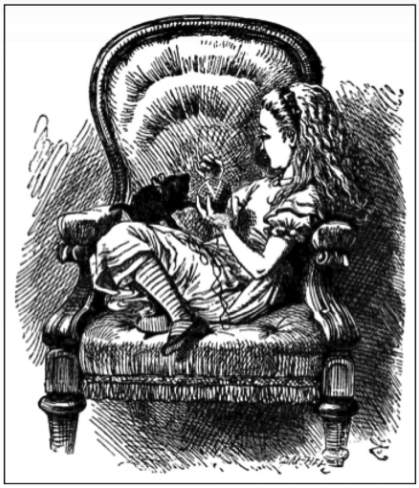
\includegraphics[width=0.9\textwidth]{Alice1}
\end{figure}
You can see Alice here playing with a ball of yarn and her kitten Dinah.
What I'd like you to imagine us doing here
is simplifying this image in different ways.
What we're going to do in particular is coarse grain the image
in the following fashion. So, imagine dividing
this image up into grids, Figure \ref{fig:alice:coarse}, and then, at each grid point here –
if we were to zoom in to this digitized
version of Tenniel's image,
say just a little on Dinah's ear here –
we'll see a little patch of that image.

\begin{figure}[H]
	\caption{Coarse Graining Alice}\label{fig:alice:coarse}
	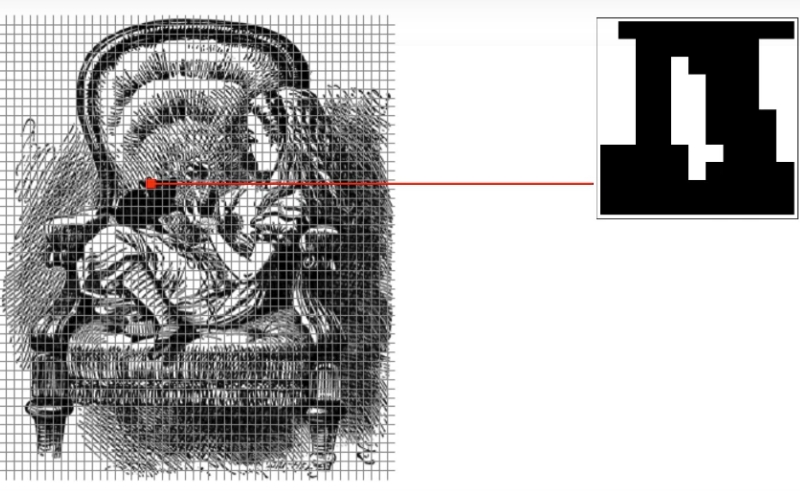
\includegraphics[width=0.9\textwidth]{Alice2}
\end{figure}
And what we're going to say
is for each of these patches,
we're going to represent them now.
Instead of all of the individual details –
the square is white, the square is black –
instead of all the individual details,
we're going to have that patch
just take a vote.
So that image, there it turns out
as majority black pixels,
and so it's going to coarse grain
to a single chunky black pixel.
And we're going to go
grid square by grid square here,
taking all of the complexity
of the image within that ten by ten chunk
and compressing it down
to a single answer:
black or white, 1 or 0.
And if we go right next door
on that image,
here's a different part of Dinah,
different part of Alice's cat,
And what we can see in Figure \ref{fig:alice:voting}
is that even though this image patch
at the fine grain level is different,
the two descriptions in the different
parts of the image are different,
our course grading majority vote
will represent them identically.

\begin{figure}[H]
	\caption{Two different configuration coarse grained identically.}\label{fig:alice:voting}
	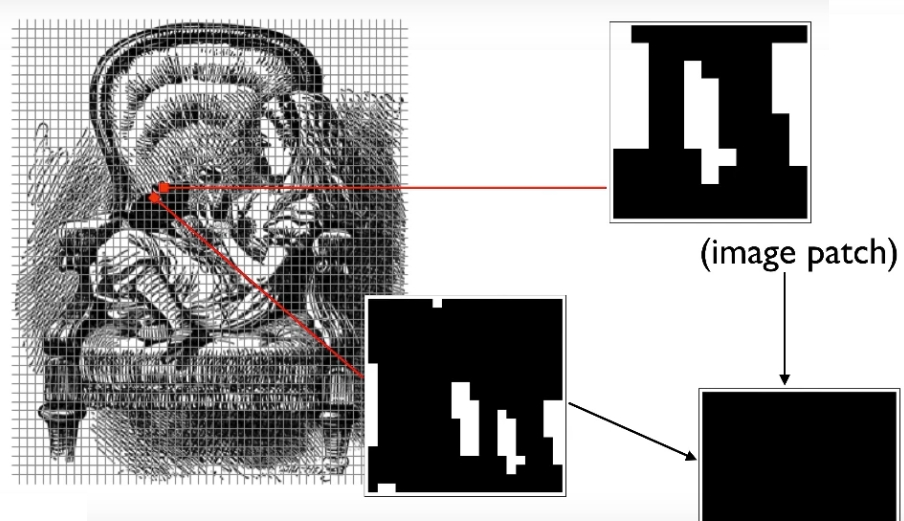
\includegraphics[width=0.9\textwidth]{Alice3}
\end{figure}
What we can see in Figure \ref{fig:alice:result:coarse:graining} is that on the left-hand side, we have the original image, and on the right-hand side
we have something that kind of looks pretty much like what
Alice sort of looks like, but we're missing quite a lot.

\begin{figure}[H]
	\caption{Majority Coarse Graining.}\label{fig:alice:result:coarse:graining}
	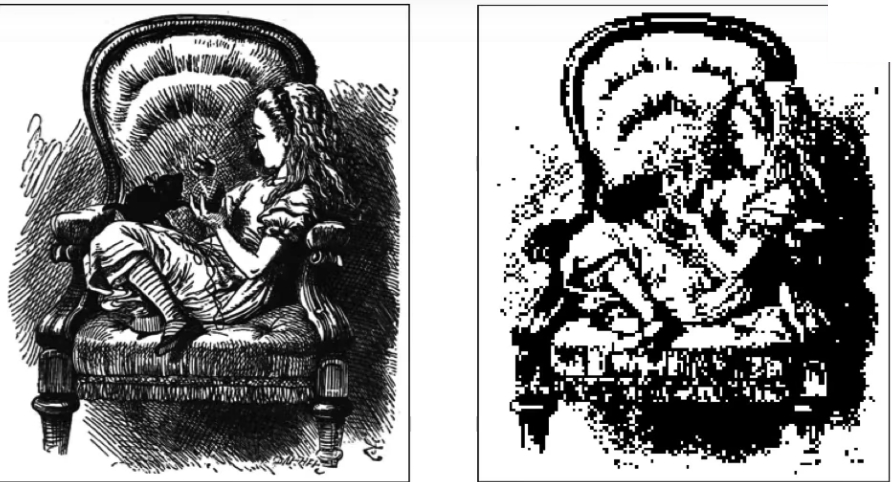
\includegraphics[width=0.9\textwidth]{Alice4}
\end{figure}

Here's another case, this is a different rule.
In this case, Figure \ref{fig:alice:result:decimation}, instead of taking the majority vote, I did what's called decimation,
at least in the literature, and this is a term that was invented
by the physicist Leo Kadanoff\cite{kadanoff2000statistical}
when he came to do this kind of coarse graining, not on pictures
from "Alice in Wonderland", but on images of atoms
being spin up or spin down, and we'll talk about that
in a later module when we come to the Ising model.
\begin{figure}[H]
	\caption{Decimation.}\label{fig:alice:result:decimation}
	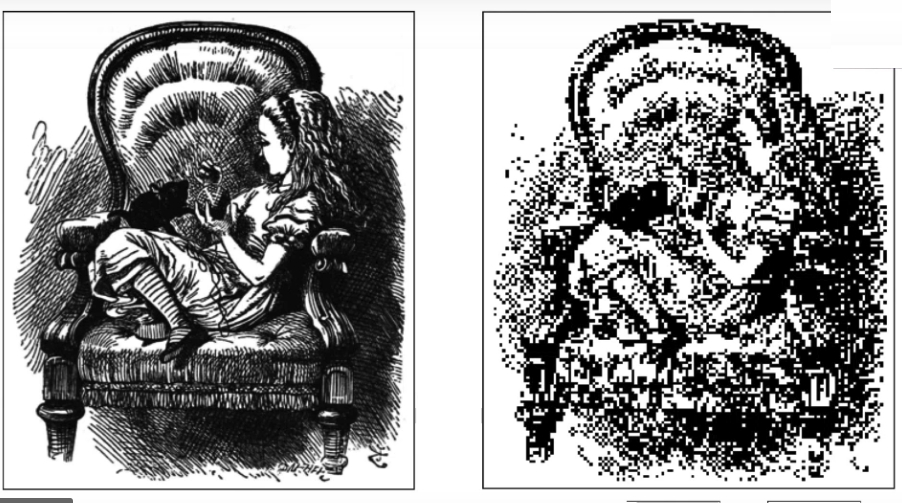
\includegraphics[width=0.9\textwidth]{Alice5}
\end{figure}

What Leo said to do is:
Don't even bother
to average over that grid square,
just take the point
in the top left corner,
and have that define it.
You can see in this case here,
if we use that decimation rule,
that same patch of die now gets mapped,
not to black, but to white.
So what I've introduced you to here
is two ways to simplify an image,
two ways to coarse grain the image,
and, of course, different images
will now coarse grain to the same thing.
I can make many microscopic changes
in Tenniel's original illustration,
and still get back
the same final image of Alice.
Of course, the microscopic changes
that my image is insensitive to,
or that, rather, my coarse graining
of the image is insensitive to,
the microscopic changes will depend upon
the coarse graining algorithm
that I choose.

So if I do the majority vote,
then I'll be able to make some changes
that won't show up,
and if I instead take
the decimation coarse graining rule,
there's a different set of changes
that I can make at the microscopic level
that will leave the system unchanged.
When we come to compress images
in the real world,
we do this quite a lot.
So, when I took this the original image,
I actually had a perfect
representation of the image,
at least at that particular scale:
I had a tiff.
The file format there means
that every single pixel in the file
is registered as either being
on or off, black or white.
On the left-hand side,
you can see what happens
if I use my unfortunately non-patented
compression algorithm,
where here, instead of compressing it
using 10x10 grids,
I do a much less aggressive compression
where I only take little 3x3 grids.
If you compare how ugly
the 10x10 grid compression is,
to the 3x3 grid compression,
you might think,
"Hey, that's pretty good."
And, in fact, by doing that,
by going from a grid that's 1x1,
by keeping track of every pixel,
and instead going to a grid that's 3x3,
I decreased the file size
by a factor of 9.
What I also can do is take that tiff file,
open it up, and max preview,
and now ask the computer
to do some coarse graining for me.
because we spend a lot of time trying
to figure out how to compress images,
how to reduce their size,
how to throw away the information
that people don't need,
in order to allow the image
to be transmitted faster,
to be stored more conveniently.
So, on the right-hand side here,
we also have a coarse graining
of the Alice image,
but now using a coarse-graining algorithm
called the JPEG.
No one's ever referred to the JPEG
as a coarse-graining algorithm,
at least they don't do it that much.
What you can see is both images
look reasonably good.
In fact, they have different properties,
so let's go zoom in here on Dinah.
What you can see on the left-hand side
is the majority vote coarse graining.
One of the features of the majority vote
coarse graining, by the way, you will see,
is that each pixel
is still a bit black or white.
If I zoom in again,
and I guess Dinah's looking here much more
like a rat now than she is like a cat,
but if you zoom in on Dinah
on the right-hand side,
you can see now the JPEG image
has made different choices
about what to keep and what to throw away.
Importantly, one of the ways
the JPEG works
is not in what we call real space,
in what the physicists call real space,
but instead what's called Fourian Space.
We'll talk a little bit more
about the distinction between
those two ways to represent an image,
but for now the simplest way
to think of it is this:
On the right-hand side,
what I did was I took the representation
of the image in the spatial field.
So, I took the entire array,
and I turned it by taking chunks
that were locally connected to each other.
I took little local chunks from the image,
and, for each of those chunks,
I did a little compression scheme.
I said all these differences here
don't matter,
you don't have to keep track
of all the either 9 or 100 pixels
within that square,

\begin{itemize}
	\item I'm going to summarize it,
	\item I'm going to coarse grain it,
	\item I'm going to simplify it,
	\item I'm going to losslessly compress it –
\end{itemize}
all these words are equivalent,
different ways and different fields,
or rather different ways
that different fields
have discovered to talk about this –
I'm going to simplify all of those pixels
in a particular way.
On the right-hand side,
what the JPEG does is the following:
it does a transformation on this image,
it represents this image
in a very different way.
What it does is it represents the image
in terms of the fluctuations
that occur in it.
So, it takes the long-wavelength
parts of the image,
the fact that in the center
it's darker than it is around the edges,
and it puts that in one pixel.
Then it also takes
the high-frequency component,
the wiggles where the image is going
from black to white
very quickly along the line.
So, here, for example, you can see
on the back of the armchair
where Alice is sitting,
very fine grid lines.
What the JPEG does, is it says,
"There's a patch here where things
are oscillating very quickly,
so I'm going to put that over
in this high-frequency part
of the image data."
It's also true of Alice's hair.
If you look at Alice's hair there,
she has these sort of kinky curls,
and those curls
have a high-frequency component
the JPEG records.
So, what the JPEG does is,
it represents that image now,
instead of representing it spatially –
so stuff on the left
is physically stuff that was on the left
in Tenniel's original recording –
it puts the low-frequency components
in one part
and the high-frequency components
in the other part.
And then it does two things.

\begin{itemize}
	\item First of all blurs them,
	so it does a kind of chunking
	coarse graining on those components,
	\item and then also it just entirely cuts off
	all the high-frequency components
	in the image –
	because there are parts of that image
	that you yourself are not sensitive to,
	and those parts are where the image starts
	fluctuating back and forth very quickly.
\end{itemize}

In fact, you can see it:
on the right-hand side,
the JPEG looks smoother
than in the compression I've done.
In fact, what's so clever about the JPEG
is it actually respects the way
in which the human eye
records information.
Amazingly enough, of course,
when the human eyes
gets data from the real world,
and makes an image
on the back of your retina,
it appears almost like a set of pixels.
But before it actually wants to transmit
that image back into your brain
to make decisions,
it does itself
a series of coarse grainings
using Gabor functions in the particular
sensitivity of the neurons.
It does a particular set
of coarse grainings
that, in fact, the JPEG knows about.
So the things that your retina
is going to throw out anyway
as it transmits it backwards,
the JPEG has already thrown out
on your behalf.
\subsection{Coarse graining part I - Clustering algorithms}

So, in the previous section,
you had an example of coarse-graining
from image compression
I showed you two different examples
of what you might call
real-space compression.
These were just things that
I made up,
that have some parallel
to what people have done
when they come to coarse-grain
a physical system.
What I did in particular
was take things
that were nearby each other in space.
I took a group
of objects, or a group of properties
of the system
that were nearby each other in space 
and I summarized them in some way.
So in the majority-rule case, for example,
all I did was, I took all the pixels
in a certain grid square, and I said, OK,
if the number of black pixels
outnumbers the number of white pixels,
then that pixel will be black,
and otherwise, it will be white.
And what I've done there, of course,
is taken a whole set of very different
grid squares, each of which
looks different,
and I mapped them all onto a single
kind of square
that only has one property, zero or one,
whereas here, in the ten-by-ten case,
there are in fact a hundred bits
of information, you might say.
So this is the general property
of coarse-graining; this is
a simple example of how we build
a function, $f$, that maps from some space $S$
to some space $S^\prime$.
This is a list of properties of, 
or this is the set of properties,
that describe the fine-grained system ---
for example, it could be the entire
productivity list,
the entire employment history
of every single person in the economy ---
and over here is a much,
usually much smaller set of quantities
that we're going to use to describe
the coarse-grained system.
Coarse-graining is something we do
all the time.
Sometimes, we make it up ahead of time.
So for example,
when we came to do the coarse-graining
of the image from Alice in Wonderland,
we just took a couple different ways
in which we thought
that simplifying the image
might work --- and of course,
what it means for it to work
is a problem that we often
don't think about 'til
right at the end, but here,
we took the majority vote.
We're saying, OK, look, you know
if this pixel, if this kind of collection
of pixels here is mostly black,
let's just call it black.
And the idea is that your eye
might not really be
sensitive to it. In the end,
what we're doing when we choose
that rule is probably having a theory
about how the eye works,
or perhaps about what we care about
when we look at an image.
Of course, you'd be crazy to
do this on a bar code or QR code,
all right,
because in that case, the device
that's scanning the image
is much more sensitive
than your eye is,
and so if you took a photograph
of a QR code,
and then coarse-grained it
in the way we did,
the QR code would probably
no longer work.
In that case, the information that
we'd be throwing out,
the distinctions between the different
elements of this set here,
that the function all maps
to the same point here,
those distinctions would have been lost.
So sometimes,
we think about the problem we want
to solve,
and invent a coarse-graining algorithm.

Other times ---
and in fact this is becoming
increasingly common ---
other times, we don't know what
the coarse-graining is when we begin,
and in fact, we'll do something
really simple, like use
a clustering algorithm.
And so a classic example of clustering
might be k-means.
So what does k-means do,
what does a k-means algorithm do?
If you haven't heard this term,
don't worry; I'm going to tell you
what it means and you can go
look it up and do it
to your heart's content.

k-means takes a set of high-dimensional
data, and because we can't afford
a high-dimensional whiteboard,
we only have two,
so what I'm going to do here is,
I'm going to put a lot of
data points here, and maybe, for example,
this axis here is height,
and this axis here is weight, OK,
and these points here refer
to individuals of a species
that you've captured in the wild,
maybe these are birds, right.
And so what k-means will do is,
it will take that rich description,
OK, where every individual is
described by a real number, OK,
on both the x and y axes here,
each bird you've caught, let's say,
has a certain height and a certain weight,
and you go out, and you sort of
laboriously, you know,
maybe you're in some tropical country,
like you're in Costa Rica or something,
which seems to be where
all the bird people go, OK,
and then you say, well, I don't know,
something's going on there,
and you hand it to k-means, which says,
oh, you know what, actually,
there's two clusters here, right?
There's this cluster, A,
and this cluster, B. And so
what k-means has done is
mapped from a two-dimensional
vector space, maybe not $R^2$
because you can't have, like, you know,
negative weights, so maybe it's just
the positive side of $R^2$, right,
it's mapped from that two-dimensional
vector space into a binary set, A and B.
So in general, when you call up
a clustering algorithm,
really what you're asking it to do
is coarse-grain my data, OK,
and then if you're a biologist,
you might be like, you know,
there's something funny, like
all the A birds, they're all female,
let's say, and all the B birds, OK,
they're all male, OK,
and now you feel really good
because in fact what you've done is,
you've discovered, using this data
here, using this rich high-dimensional
data, you've discovered a simple
low-dimensional explanation
for what's happening.
Why do birds have different weights?
Well, you know, the main thing is,
is if they're women, or if they're men,
if they're male or female.
So, clustering is sort of an automated way
to have the data suggest to you
what a good coarse-graining might be.
You may have noticed, of course, that
in fact, k-means operates with a notion
of closeness just as the
Alice in Wonderland coarse-graining did.
In both cases, we were saying that
things that were near each other, OK,
should probably be described by
a single description, right?
All these points here get
the description A; all these points here
get the description B.
k-means is in fact an example of
what we call a hard clustering, OK,
and in this case here it says that
each point is uniquely assigned
to a single cluster, and this kind of
hard clustering is a form of
coarse-graining, is the easiest to
understand, and we'll give an example of,
in particular, how hard clustering plays
a central role in information theory. OK.

There are other clustering algorithms
that give what are called soft clusterings,
and the most closely related
soft clustering algorithm to the
k-means one is called the GMM,
or the Gaussian mixture model.
And in fact the GMM is very similar
to k-means. What it does is, it takes
high-dimensional data, a vector of
high-dimensional data, or rather a set
of vectors of high-dimensional data,
right, each point referring to
a particular observation, and what the GMM
does is says, oh, you know, it looks like
this could be described as, like,
you're kind of drawing from two
Gaussians, right, the Gaussians
have a particular center, right,
they have a particular variance
and covariance matrix,
so they kind of, like,
these little sausages that lie here,
right, OK, and so what the GMM does is,
it produces a Bayesian model
of the way your data might have been
created, OK, and then for each point here,
it tells you the probability that that point
was drawn either from this Gaussian ---
we'll call that $G_1$ --- or this
Gaussian --- call it $G_2$.
So in fact, in this case, it's giving you
not a unique assignment, but it's
giving you a sort of probabilistic
assignment. In particular, it's mapping
this two-dimensional vector space ---
and let's say it finds two clusters ---
it's mapping that two-dimensional
vector space into the, sorry,
into the interval [0, 1], which you can
think of here as the probability
that the point was drawn from cluster A.
So this point here, right, really centered
to the first cluster, that would have a
very high probability of being a member
of $G_1$ and a much lower probability of
being a member of $G_2$.
So these are subtly different concepts
here --- there's the hard clustering case
when it takes each point and says, OK,
here is the coarse-grained category
you belong to. Just as in the case of the
Alice in Wonderland algorithm, what
we did was, we took that little
grid square, that ten-by-ten grid,
and we say, OK, you're majority zero,
therefore you belong to
the category zero, you're majority one,
you belong to the category one.
The soft clustering is a little weaker,
right; it sort of avoids
making a decision. You'll encounter,
probably in your own research,
different kinds of clustering algorithms,
different kinds of clustering choices.
People tend to prefer hard clustering,
because you don't have to think as hard
when you work with it.

\subsection{Coarse graining part II - Entropy}

The last thing I promised you
was to tell you how coarse graining
fit into the story of information theory.
So, even if you have not discovered
the information theory lectures,
you will get
a very brief introduction to it.

Let's imagine that we have some process,
let's say with 26 options:
there's the probability
that the process emits A,
the probability that the process emits B,
all the way down to the probability
that the process emits Z.

What information theory does,
one of the canonical questions
it asks, is:
How much information
is in that process?
This term also comes up:
How much entropy is in the process?
Another term is: How much uncertainty is in the process?

A process that has higher uncertainty –
in this case here, a process
when you stick your hand in the bag,
you don't know if you're going
to get an A or B or C
all the way down to Z –
a process that is more uncertain
has higher entropy,
and has higher information.

Claude Shannon invented a way
to measure, or to quantify,
to turn this big list of numbers,
this big list of probabilities,
into a single number which he then called
the uncertainty of the process itself.
He called that function H, the fundamental quantity
of information theory:

\begin{align*}
H \triangleq \sum p_i \log_2(p_i) \numberthis \label{eq:shannon:entropy}
\end{align*}

One of the questions you might have is:
How did Shannon derive it?
What he did was,
he came up with a series of axioms
that he wanted this function to satisfy.

\begin{itemize}
	\item First of all, the maximum uncertainty that this distribution can have
	is if each of these probabilities is equally likely.
	So if the probability of A is 1 in 26, 	the probability of B is one in 26,
	and all the way down to Z, 	that should mean, if that's the case,
	you should be maximally uncertain 	about what's going to happen.
	That's the first thing he said.	The more uniform ... rather ...
	if it's perfectly uniform, 	the probabilities are perfectly uniform,
	that should be the condition of maximum uncertainty.
	\item He also wanted it to be symmetric,
	he didn't want it to discriminate
	between each of these different variables.
	So, for example,
	a probability distribution
	where A and B both had probability 0.5,
	and everything else was 0,
	should have the same uncertainty
	as the distribution where the probability
	of Y and Z are both 0.5,
	and everything else was 0.
	He didn't want to discriminate
	between the different options,
	and, for this reason, information theory
	is sometimes called a syntactic theory.
	So, well, that makes sense, right?
	If you shuffle these around,
	that should be good, right?
	It doesn't matter
	what these probabilities attach to.
	And the second thing
	is conditioned of maximal uncertainty.
	\item The coarse-graining axiom says the following: let's say you have three options, \{A,B,C\}.
	And, in this case here, for simplicity,
	we'll assume that these are independent
	in the sense that if I get an A,
	it doesn't affect
	what I'm going to get next;
	So, Shannon said, okay
	the entropy of that system
	should be equal given by (\ref{eq:coarse_grain_axiom}): the entropy of the coarse-grain system, plus the weighted entropies of those fine-grain distinctions.
\end{itemize}



\begin{align*}
H (P_A,P_B,P_C) = H(P_A,P_{B,C}) + (P_A+P_B)H(B,C) \numberthis \label{eq:coarse_grain_axiom}
\end{align*}
And once you demand
that this property here be obeyed, then you recover Shannon's
original formulation of entropy--(\ref{eq:shannon:entropy}). And it turns out
that this formulation is now unique: there is no other functional form
for how to convert a list of probabilities into a number describing uncertainty,
that obeys the condition of a maximum uncertainty, that obeys the syntax property
of being able to shuffle and get the same answer,
and that, finally, obeys Shannon's coarse-graining axiom. If you enforce all of those, this is the final formula that you're left with, no other formula will do.

And one of the very nice things about this
is that the course-graining axiom shows you how,
when you coarse-grain a system, the uncertainty,
the information that you have, goes down.
So let's say that instead of representing
the system like this \{A,B,C\},
I broke it up into these two pieces here, \{A,\{B,C\}\}
coarse-grained uncertainty,
and then a fine-grained uncertainty,
where I split the \{B,C\} case;
in that case, (\ref{eq:coarse_grain_axiom})  becomes (\ref{eq:coarse_grain}):
\begin{align*}
H (P_A,P_B,P_C) \ge& H(P_A,P_{B,C})  \numberthis \label{eq:coarse_grain}\\
H (P_A,P_B,P_C) >& H(P_A,P_{B,C})\text{, if there's some possibility of B and C}
\end{align*}

So, in this first module what have we done? I've given you a short introduction
to the idea of renormalization through the example of the microeconomics story. You have a microeconomic account of the world,
a very detailed description of what people are doing
that you then coarse grain to a macroeconomic account.
That coarse graining generally erases distinctions:
instead of distinguishing case B from case C,
you say, "Ah, you know what? They're pretty much the same."
We had an example of that coarse-graining property
in the case of coarse-graining the image of Alice in Wonderland.
And there, I actually gave you three examples,
majority rule coarse graining, decimation coarse graining,
and a more complicated, sort of Fourier space kind of coarse graining,
called the JPEG, which of course is now in so much use
that your computer has a special chip that does JPEG decompression.
So, I gave you an example of how coarse graining worked,
and, in this final part of the lecture of this first part of the module,
what I've done is tell you a little bit about
how coarse graining plays a central role in information theory.

But coarse graining is not enough. It's not enough
just to simplify the world, because, in the end, what scientists do
is something more than just create JPEGs. What a biologist does
is something more than just clustering – or rather you hope a biologist is doing
something more than just clustering, although you should check the literature
because sometimes they don't. And, in fact, many scientists
fall victim to this: they think that if you have a compressed,
efficient description of the world then you're done.

But you're not done, because what you want to do
with that compressed description is make predictions, produce explanations,
try to describe, but not just describe: try to explain what happened before
and what's going to happen next. And in order to do that,
you need a theory. And what renormalization does,
is it says, "Great, congratulations, you've constructed a coarse graining,
now, how is the theory connecting those different coarse-grained states,
how is that theory related to the one at the fundamental level?

How can you go, in other words, or rather what happens when you take
a full economic and psychological theory of the world
and course-grain it to macroeconomics? What happens when the macroeconomist
then tries to build a theory that relate his coarse-grain quantities?"
And so, in the next module, we will give you your first simple example
of how theories about the world change when the objects
that they describe simplify.

References: \cite{dedeo2018information,dedeo2013bootstrap,dedeo201716}

\section{Markov Chains}

\subsection{Markov Chains}

\subsection{Mathematics of coarse grained Markov chains}

\subsection{Mathematics of Coarse grained Markov Chains: The General Case }

\subsection{A puzzle: origin of the slippy counter}

\subsection{Where we are so far}

\cite{dedeo2016conflict}

\section{Cellular Automata}

\subsection{Cellular Automata: an Introduction}

\subsection{Israeli and Goldenfeld; projection and commuting diagrams }

\subsection{Networks of Renormalization}

\cite{israeli2004computational,israeli2006coarse,dedeo2018origin}
\section{Ising Model}

\subsection{Fixing a projection: From CA’s to Ising}
Effects of coarse graining in time:
\begin{itemize}
	\item Markov Chain--everything flows to lower dimensional subspace; first example of fixed point.
	\item Cellular Automata--in order to stay within same model class, forced to coarse grain in space also. Can coarse grain universal rule 110, but projection is practically trivial. Non locality arises. 
\end{itemize}

When we coarse-grain Ising model we also lose locality!
\subsection{Introduction to the Ising Model}

Describe atoms on a lattice, e.g. 2D. Each atom has spin $\sigma=\pm 1$. Things which are near each other "want" to be like each other. The probability of a configuration is given by:

\begin{align*}
P(\{\sigma_i\}) =& \frac{e^{\beta \sum_{i,j} J_{i,j} \sigma_i \sigma_j}}{Z(\beta)}\text{, where} \numberthis \label{eq:coarse_ising:P} \\
J_{i,j} =& 1,\text{if $i$ and $j$ are neighbours (connection or adjacency matrix)}\\
=& 0 \text{ otherwise.}\\
\beta =& \frac{1}{T}\\
Z(\beta) =& \text{ the partition function (normalization constant).}
\end{align*}

\begin{itemize}
	\item "lattice" could be a network;
	\item used also to model alignment of opinions.
\end{itemize}

Start with a very simple course-graining, where we ignore one node, A say, only, as shown in Figure \ref{fig:ising-coarse1}.

\begin{figure}[H]
	\caption{Simple coarse graining, ignoring $\sigma_A$}\label{fig:ising-coarse1}
	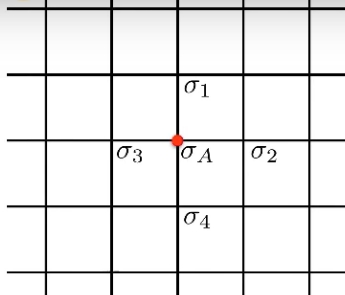
\includegraphics[width=0.9\textwidth]{ising-coarse1}
\end{figure}

\begin{enumerate}
	\item pull out the term in the sum with $\sigma_A$
	\item average out ("trace out") $\sigma_A$
\end{enumerate}
Then (\ref{eq:coarse_ising:P}) becomes:
\begin{align*}
P(\{\sigma_i\}) =& \frac{\big[\sigma_1\sigma_A + \sigma_2\sigma_A + \sigma_2\sigma_A + \sigma_4\sigma_A\big]B}{Z(\beta)} \text{ for fixed $\sigma_A$, where}\\
B =& e^{\sum e^{\beta \sum_{i,j \ne A} J_{i,j} \sigma_i \sigma_j}}\\
\sum_{\sigma_A=\pm 1} P(\{\sigma_i\}) =& \big[e^{\beta(\sigma_1+\sigma_2+\sigma_3+\sigma_4)} + e^{-\beta(\sigma_1+\sigma_2+\sigma_3+\sigma_4)}\big]  \frac{B}{Z(\beta)}\\
=& 2 \cosh({\beta(\sigma_1+\sigma_2+\sigma_3+\sigma_4)})   \frac{B}{Z(\beta)}\\
=& e^{\log{\cosh({\beta(\sigma_1+\sigma_2+\sigma_3+\sigma_4)})}} \frac{B}{Z^\prime(\beta)} \text{, absorbing $2$ in $Z^{\prime}$.} \numberthis \label{eq:coarse_ising:P2}
\end{align*}

Comparing (\ref{eq:coarse_ising:P}) and (\ref{eq:coarse_ising:P2}), we see that coarse graining has complicated equation. However, Figure \ref{fig:ising-cosh} suggests a way forward.

\begin{figure}[H]
	\caption{Simple coarse graining: analyzing the $\cosh$ term.}\label{fig:ising-cosh}
	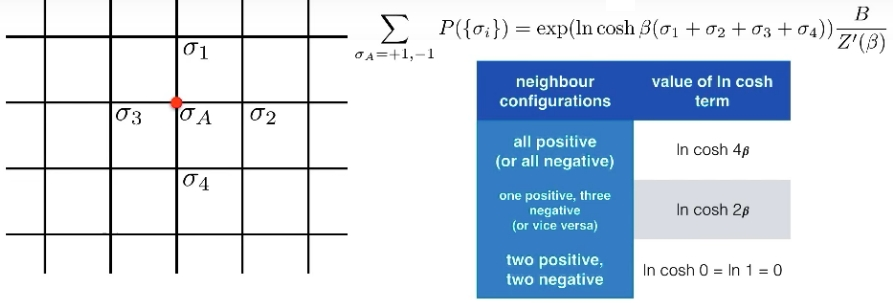
\includegraphics[width=0.9\textwidth]{ising-cosh}
\end{figure}

We find that (subject to a constant factor, which can be absorbed in partition function):
\begin{align*}
\sum_{\sigma_A=\pm 1} P(\{\sigma_i\}) =&e^{S_2 (\sigma_1\sigma_2 + \sigma_1\sigma_2+ \sigma_2\sigma_3 + \sigma_2 \sigma_4 + \sigma_3 \sigma_4 +\sigma_4 \sigma_1) + S4 \sigma_1 \sigma_2 \sigma_3 \sigma_4} \text{,where} \numberthis \label{eq:coupled:sigmas}\\
S_2 =& \frac{1}{8} \ln{\cosh{4\beta}} \tag*{pairwise interactions}\\
S_4 =& S_2 - \frac{1}{2} \ln{\cosh{2\beta}} \tag*{quartet interaction.}
\end{align*}

Notice that (\ref{eq:coupled:sigmas}) couples $\sigma_1, \sigma_2, \sigma_3, \& \sigma_4$! This includes longer range couplings, such as $\sigma_2, \sigma_3$, plus the quartet!

\subsection{Coarse-graining the Lattice}

This is just a summary of previous section.

\subsection{Inducing Quartets \& Commutation Failure}

Figure \ref{fig:ising-decimation}\cite{aoki2014domain} shows a decimation of the entire lattice. It exhibits 3 types of coupling:

\begin{enumerate}
	\item the survivors form a new lattice, rotated \ang{45}, with coupling $2S_2=\frac{1}{4} \log{\cosh{4 \beta}}$\label{item:coupling1}
	\item long range couplings, over a deleted $S_A$,  $S_2=\frac{1}{8} \log{\cosh{4 \beta}}$\label{item:coupling2}
	\item quartet couplings $S4=\frac{1}{2} \log{\cosh{2\beta}}$\label{item:coupling3}
\end{enumerate}

\begin{figure}[H]
	\caption{Coarse-graining the Lattice}\label{fig:ising-decimation}
	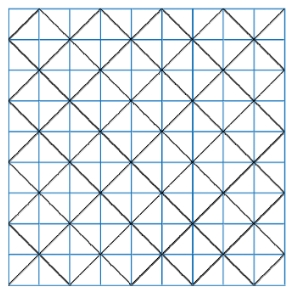
\includegraphics[width=0.9\textwidth]{isinng-decimation}
\end{figure}

If we can ignore couplings \ref{item:coupling2} \& \ref{item:coupling3} We have transformed original lattice with coupling $\beta$ into one with coupling \ref{item:coupling1}: $\frac{1}{4} \log{\cosh{4\beta}}$.

\begin{thm}[Monotonicity of Ising Decimation]
	$\beta > 0 \implies \frac{1}{4} \log{\cosh{4\beta}} < \beta$
\end{thm}

\begin{proof}
	\begin{align*}
	\frac{1}{4} \log{\cosh{4\beta}} =& \frac{1}{4} \log{\frac{e^{4\beta} + e^{- 4 \beta}}{2}}\\
	<&  \frac{1}{4} \log{\frac{e^{4\beta} }{2}}\\
	<& \frac{1}{4} \log{e^{2\beta} } \\
	<& \frac{1}{2} \frac{1}{\cancel{2}} \cancel{2} \beta\\
	<& \beta
	\end{align*}
\end{proof}

Since coupling decreases as we zoom out, we are less and less likely to see big domains that are aligned the same way. NB: this is not the same as previous Markov and Cellular automata, where we performed exact renormalization; this is approximate.

This is a bad approximation. We can do better by ignoring coupling \ref{item:coupling3} (quartet) and lumping \ref{item:coupling1} and \ref{item:coupling2}, new coupling $\frac{3}{8} \log{e^{2\beta} }$. This is a heuristic, but, apparently, doesn't work too badly.


See also \cite[Chapter 14]{kadanoff2000statistical}
\subsection{Finding Fixed Points}
\subsection{Ising Model Simulations}
\cite{dedeo2012dynamics}

\section{Krohn-Rhodes Theorem}

\subsection{Poking the Creature: An Introduction to Group Theory}

\subsection{Irreversible Computations, Forgetful Computers and the Krohn-Rhodes Theorem }

\section{A Classical Analogy for Renormalization in Quantum Electrodynamics}
\subsection{From Quantum Electrodynamics to Plasma Physics }
\subsection{The Thermal Physics of Plasma}
\subsection{How does a particle move the plasma?}
\subsection{Charge Renormalization and Feedback}

\section{Conclusion: The Future of Renormalization \& Rate Distortion Theory}

% bibliography go here

\bibliographystyle{unsrt}
\addcontentsline{toc}{section}{Bibliography}
\bibliography{../complexity}


\end{document}
